\documentclass[11pt]{article}
\usepackage{textcomp}
\usepackage{longtable}
\usepackage{graphicx}
\usepackage{subcaption}
\usepackage{listings}
\usepackage{color}
\usepackage{paralist}
\usepackage[hyphens]{url}
\usepackage{geometry}
\usepackage{wrapfig}

\geometry{a4paper, left=25mm, top=25mm}

\definecolor{codegreen}{rgb}{0,0.6,0}
\definecolor{codegray}{rgb}{0.5,0.5,0.5}
\definecolor{codepurple}{rgb}{0.58,0,0.82}
\definecolor{backcolour}{rgb}{0.95,0.95,0.92}

\lstdefinestyle{mystyle}{
    backgroundcolor=\color{backcolour},
    commentstyle=\color{codegreen},
    keywordstyle=\color{magenta},
    numberstyle=\tiny\color{codegray},
    stringstyle=\color{codepurple},
    basicstyle=\footnotesize,
    breakatwhitespace=false,
    breaklines=true,
    captionpos=b,
    keepspaces=true,
    numbers=left,
    numbersep=5pt,
    showspaces=false,
    showstringspaces=false,
    showtabs=false,
    tabsize=2
}

\lstset{style=mystyle}


\graphicspath{ {Images/}{Graphs/} }
\author{Eugene Valetsky\\ \and Supervisor: Dr Tim Baker}
\title{Unmanned Aerial Systems}

%%%%%%%%%%%%%%%%%%%%%%%%%%%%%%%%%%%%%%%%%%%%%%%%%%%%%%%%%%%%%%%%%%%%%%%%%%%%%%%
% DOCUMENT
%%%%%%%%%%%%%%%%%%%%%%%%%%%%%%%%%%%%%%%%%%%%%%%%%%%%%%%%%%%%%%%%%%%%%%%%%%%%%%%
\begin{document}
\maketitle
\tableofcontents
\newpage

\documentclass[11pt]{article}

\usepackage{geometry}
\geometry{a4paper, left=25mm, top=25mm}

\title{\vspace{-2em}Unmanned Aerial Systems}
\author{Eugene Valetsky \and Supervisor: Dr Tim Baker}
\date{}

\begin{document}
\maketitle

\documentclass[11pt]{article}

\usepackage{geometry}
\geometry{a4paper, left=25mm, top=25mm}

\title{\vspace{-2em}Unmanned Aerial Systems}
\author{Eugene Valetsky \and Supervisor: Dr Tim Baker}
\date{}

\begin{document}
\maketitle

\documentclass[11pt]{article}

\usepackage{geometry}
\geometry{a4paper, left=25mm, top=25mm}

\title{\vspace{-2em}Unmanned Aerial Systems}
\author{Eugene Valetsky \and Supervisor: Dr Tim Baker}
\date{}

\begin{document}
\maketitle

\input{Sections/Abstract.tex}

\vspace{2em}
\small
\emph{I, Eugene Valetsky, confirm that the work to be presented at the 2nd panel meeting, and whose abstract is given above, is my own. Where information has been derived from other sources, I confirm that this is indicated in the presentation.}

\end{document}


\vspace{2em}
\small
\emph{I, Eugene Valetsky, confirm that the work to be presented at the 2nd panel meeting, and whose abstract is given above, is my own. Where information has been derived from other sources, I confirm that this is indicated in the presentation.}

\end{document}


\vspace{2em}
\small
\emph{I, Eugene Valetsky, confirm that the work to be presented at the 2nd panel meeting, and whose abstract is given above, is my own. Where information has been derived from other sources, I confirm that this is indicated in the presentation.}

\end{document}


\section{Introduction}
The Unmanned Aerial System (UAS) Challenge was launched by the Institution of Mechanical Engineers (IMechE) in 2014 `with the key objectives of developing professional engineers and inspiring the next generation'\cite{IMechE_about_uas}. The main goal is to design and build a UAS in order to autonomously deliver humanitarian aid such as medical supplies in a disaster zone. This requires a broad range of skills, from project management to airframe design to avionics system programming. To add to the challenge there is a strict weight limit and stringent safety regulations. Working together with another student, Ismail Ahmad, our goal is to follow the design and build cycle all the way through to competing at the IMechE UAS competition in June 2018.

One of the greatest individual challenges as part of the project is creating an autonomous flight system. The UAS must be capable of quickly and safely navigating to and locating a target using computer vision, dropping a payload accurately, and returning to base. This requires an understanding of the UAS’s flight dynamics as well as good programming and wiring capabilities. This is the aspect that I will be focusing on for my individual project, although I will be assisting with many parts of the project.

\section{Design}
\subsection{Concept}
The concept for our UAS uses a hybrid symbioisis between a \emph{Micro Jet Engine}, henceforth refered to as MJE, and an external multi-rotor. The MJE is gimballed to always remain vertical and only provides lift, while the multirotor rotates around it providing stabilisation and control. This configuration means that standard quadcopter flight control software can be used rather than needing to come up with custom architecture.

The MJE provides a higher thrust to weight ratio than the equivalent electric motors and batteries (see Appendix \ref{app:thrust_to_weight}). It does this without introducing the vibration issues of a piston engine, which would seriously impact stability and control on such a lightweight design. With the current MJE and electric motors we hope to lift a payload of 3kg while remaining under the 6.9kg weight limit.
% TODO: 3 or 4 kg?

Flight control will be handled with a Pixhawk running the PX4 flight stack. This will be coupled to a companion computer running software based on the DroneKit SDK, communicating with the PixHawk using the MAVLink protocol. The companion computer is responsible for communication, waypoint navigation, and target location and tracking using computer vision. It then communicates where to go to the PixHawk.

\section{Simulation: System Plausibility}
\subsection{Concept}
One of the main concepts behind the UAS concept is the idea that, if the MJE is gimballed to remain vertical, and its thrust vector is through the center of gravity of the vehicle, it exerts no horizontal forces or moments on the rest of the vehicle. This means its effect on the stability and control of the vehicle can be ignored. In turn, this means that regular quadcopter flight control software can be used, such as the PX4 flight stack.

Being able to use PX4 firmware running on a Pixhawk is crucial. The UAS will come to cost approximately \pounds2,500. Using home-made flight control software is therefore extremely risky. PX4, on the other hand, is a project that has been worked on by thousands of people for years, and is infinitely more reliable than anything we could put together from scratch.

Therefore, it was decided to build a simulation to test the validity of the concept that the MJE can be ignored.

\subsection{Equations of Motion}
The vehicle is split into two sections, the outer quadcopter frame, \emph{Quad}, and the gimballed section containing the MJE, \emph{Jet}. A cartesian reference frame was chosen, with the xy plane being the horizontal plane and z being height. +x is right, +y is forward, +z is up. A rotation about the x axis is pitch, about the y axis is roll, and about the z axis is yaw. These are labelled $\theta_x, \theta_y,$ and $\theta_z$ for the quad and $\phi_x, \phi_y,$ and $\phi_z$ for the jet respectively.

The gimbal is controlled by two servos, one moving the gimbal in roll and one in pitch. (There is no need for yaw control of the jet.)  Note that this means $\theta_z = \phi_z$.

The multirotor uses the 'quad-x' configuration, as shown below. Note that motors 1 and 3 spin clockwise, and motors 2 and 4 spin anticlockwise.
% TODO: add a diagram here.

\subsubsection{Forces}
Our gimbal design will transmit forces, but not moments. Thus, from a forces perspective, the vehicle is treated as a single unit. The total mass is
\begin{equation}
    M_{TOT} = \underbrace{\rho\pi h (r_2-r_1)}_{Frame} + 4\cdot\underbrace{\rho\pi L r_r^2}_{Rods} + 4\cdot\underbrace{M_M}_{Motors} + 2\cdot\underbrace{M_G}_{Servos} + \underbrace{M_J}_{Jet} \label{eqn:total_mass}
\end{equation}
The forces acting on the system are:
\begin{eqnarray}
    F_x = (F_{M1} + F_{M2} + F_{M3} + F_{M4})\cdot\sin{\theta_x}\cdot\cos{\theta_z} +  F_J\cdot\sin{\phi_x}\cdot\cos{\phi_z} \\
    F_y = (F_{M1} + F_{M2} + F_{M3} + F_{M4})\cdot\sin{\theta_y}\cdot\cos{\theta_z} +  F_J\cdot\sin{\phi_y}\cdot\cos{\phi_z} \\
    F_z = (F_{M1} + F_{M2} + F_{M3} + F_{M4})\cdot\cos{\theta_x}\cdot\cos{\theta_y} +  F_J\cdot\cos{\phi_x}\cdot\cos{\phi_y}
\end{eqnarray}

\subsubsection{Quad Rotation}
The quad is modeled as an inner thin, hollow cylinder, the \emph{frame}, with four cyclindrical rods, the \emph{arms}, extending outwards. The motors are point masses on the ends of the arms. It is assumed to be constructed of aircraft-grade aluminium. This results in the following inertias about the three defined axes:
\begin{eqnarray}
    % TODO: seperate symbols for quad and jet inertia
    I_{Qx} = I_{Qy} & = & \underbrace{\frac{\pi \rho h_F}{12}(3(r_2^4-r_1^4) + h_F^2(r_2^2-r_1^2))}_{Frame} \nonumber \\ & + & 4 \cdot \underbrace{\sin 45 \cdot (\frac{M_R L_R^2}{12}+M_R(r_2+\frac{L_R}{2})^2)}_{Rods} \nonumber \\ & + & 4 \cdot \underbrace{\sin 45 \cdot M_M(r_2+L)^2}_{Motors} \\
    I_{Qz} & = & \underbrace{\frac{\pi \rho h_F}{2}(r_2^4-r_1^4)}_{Frame} \nonumber \\ & + & 4 \cdot \underbrace{\frac{M_RL_R^2}{12} + M_R(r_2+\frac{L_R}{2})^2}_{Rods} \nonumber \\ & + & 4 \cdot \underbrace{M_M(r_2+L)^2}_{Motors}
\end{eqnarray}
% TODO: add a diagram here

On the quad, the gimbal servos exert offset moments about the z-axis. This results in the following equations:
\begin{eqnarray}
    \tau_{Qx} = (-F_{M1} - F_{M2} + F_{M3} + F_{M4})\cdot(L_R + r_2)\cdot \cos{45} \\
    \tau_{Qy} = (F_{M1} - F_{M2} - F_{M3} + F_{M4})\cdot(L_R + r_2)\cdot \cos{45} \\
    \tau_{Qz} = (F_{M1} - F_{M2} + F_{M3} - F_{M4})\cdot(L_R + r_2)\cdot \cos{45} + \tau_{Gx}\cdot r_1 + \tau_{Gy}\cdot r_1
\end{eqnarray}

\subsubsection{Jet Rotation}
Since $\theta_z = \phi_z$, we are only interested in the rotation of the jet about the x and y axes. Since there is a rigid linkage between the servo and the gimbal, the position of the servo is proportional to the rotation of the jet.

The jet is modelled as a cylinder. However, it does not rotate about its origin in x and y, but about the appropriate servo. Including the inertia of the servos themselves (see Appendix \ref{app:servo_info}) results in the following inertias:
\begin{equation}
    I_{Jx} = I_{Jy} = 3.89\times10^{-4} + M_J\cdot3r_J^2 + h_J^2 + M_Jl_c^2
\end{equation}

We know from Appendix \ref{app:servo_info} the maximum torque the servo can exert is 0.34 kg-m. The actual torque exerted is controlled by a PID controller in order to keep the jet vertical.

\subsection{PID Control}
8 PID controllers are needed in total: 3 position and 3 angle controllers for the quad, and 2 angle controllers for the jet gimbal. These controllers use the standard PID control logic:
\begin{eqnarray*}
    error = setpoint - actual\ value \\
    integral = integral + (error \times time\ period) \\
    derivative = (error - previous\ error)/time \\
    output = kP \times error + kI \times integral + kD \times derivative
\end{eqnarray*}
where kP, kI, and kD are constants to be optimised.

\subsubsection{Quad Control}
In a real quadcopter, the controller sends a signal to an \emph{electronic speed control} (ESC), which in turn sends a \emph{pulse width modulation} (PWM) signal to the motor, controlling its speed. In this model this has been simplified, such that the controller output directly controls the force exerted by the motors.

\begin{center}
\begin{tabular}{cc}
    $SP_x$ & Quad X position controller setpoint \\
    $SP_y$ & Quad Y position controller setpoint \\
    $SP_z$ & Quad Z position controller setpoint \\
    $SP_{\theta_x}$ & Quad X angle controller setpoint \\
    $SP_{\theta_y}$ & Quad Y angle controller setpoint \\
    $SP_{\theta_z}$ & Quad Z angle controller setpoint \\
    $O_x$ & Quad X position controller output \\
    $O_y$ & Quad Y position controller output \\
    $O_z$ & Quad Z position controller output \\
    $O_{\theta_x}$ & Quad X angle controller output \\
    $O_{\theta_y}$ & Quad Y angle controller output \\
    $O_{\theta_z}$ & Quad Z angle controller output \\
\end{tabular}
\end{center}

The controllers work in sequence, with the x and y position controllers determing the setpoint of the x and y angle controllers. The Z axis controller is independent.
\begin{eqnarray}
     O_x = SP_{\theta_x} \nonumber \\
     O_y = SP_{\theta_y} \nonumber \\
     F_{M1} = O_z - O_{\theta_x} + O_{\theta_y} + O_{\theta_z} \\
     F_{M2} = O_z - O_{\theta_x} - O_{\theta_y} - O_{\theta_z} \\
     F_{M3} = O_z + O_{\theta_x} - O_{\theta_y} + O_{\theta_z} \\
     F_{M4} = O_z + O_{\theta_x} + O_{\theta_y} - O_{\theta_z}
\end{eqnarray}

\subsubsection{Jet Gimbal Control}
Servos are controlled by sending an electronic signal to tell them what position to rotate to.

\begin{center}
\begin{tabular}{cc}
    $SP_{\phi_x}$ & Jet X angle controller setpoint \\
    $SP_{\phi_y}$ & Jet Y angle controller setpoint \\
    $O_{\phi_x}$ & Jet X angle controller output \\
    $O_{\phi_y}$ & Jet Y angle controller output \\
\end{tabular}

\begin{eqnarray}
    \tau_{Jx} = O_{\phi x} \\
    \tau_{Jy} = O_{\phi y}
\end{eqnarray}
\end{center}

% NOTE: need to check if this is correct, can a simplify a servo this way?

\subsection{Programming}
The simulation itself was written in Processing. This is a language originally based on Java that is designed for ease of programming, especially with regards to displaying graphical elements. It was chosen over using MATLAB due to the author's increased familiarity with it, and the fact that this simulation has no need of advanced mathematical capability - there are no complex differential equations or matrix operations.

The program was built up in stages, with the physics of each stage checked before adding complexity. As far as possible, good object-oriented programming practice has been followed.

The quad section was implemented first. A controller was first tested solely in the z direction, and the response was used to calibrate PID values for the z controller. Angular controllers were then implemented, tested, and calibrated, before finally introducing x and y position controllers.

Testing involved flying a simple path: takeoff to 10m, a square path (10m north, 10m east, 10m south, 10m west), and then landing. This gave the results seen in Figure \ref{fig:square_path_quad_only}. It can be seen that there is an oscilliation in x and y position. It proved difficult to eliminate, due to the not straightforward interaction of position and angle PID values. This, however proved not to be a problem. It can be seen in Figure \ref{fig:square_path_w_jet} that the addition of the jet has, likely due to the added mass, damped out the oscillations in x and y position. It has also added an overshoot in z and a steady state error in x and y, but this can be corrected by fine-tuning of PID values. The flight time has also increased but this is to be expected with greater mass. In Figure \ref{fig:square_path_w_jet_angle} we can see how the quadcopter changes angle about the x axis, and how the jet initially starts to move in that direction but is quickly brought back to the vertical by the servo.

\begin{figure}[p]
    \begin{subfigure}{0.48\textwidth}
        \includegraphics[width=\linewidth]{square_path_quad_only}
        \caption{Quad Only}
        \label{fig:square_path_quad_only}
    \end{subfigure}\hspace*{\fill}
    \begin{subfigure}{0.48\textwidth}
        \includegraphics[width=\linewidth]{square_path_w_jet}
        \caption{With Jet}
        \label{fig:square_path_w_jet}
    \end{subfigure}
    \medskip
    \begin{subfigure}{0.48\textwidth}
        \includegraphics[width=\linewidth]{square_path_w_jet_angle}
        \caption{With Jet}
        \label{fig:square_path_w_jet_angle}
    \end{subfigure}\hspace*{\fill}
    \begin{subfigure}{0.48\textwidth}
        \includegraphics[width=\linewidth]{square_path_limited_servos}
        \caption{With Refiments}
        \label{fig:square_path_limited_servos}
    \end{subfigure}
    \medskip
    \begin{subfigure}{0.48\textwidth}
        \includegraphics[width=\linewidth]{square_path_limited_servos_angle}
        \caption{With Refiments}
        \label{fig:square_path_limited_servos_angle}
    \end{subfigure}\hspace*{\fill}
    \begin{subfigure}{0.48\textwidth}
        % \includegraphics[width=\linewidth]{pic6.pdf}
        % \caption{Sixth subfigure}
        % \label{fig:f}
    \end{subfigure}

    \caption{Simulation of a Square Path}
    \label{fig:Square Path}
\end{figure}


\subsection{Refiment}
It was realised that the mass of the quad had been implemented incorrectly ($r_r$ had not been squared and the rod mass and motor mass had not been multiplied by 4 in equation \ref{eqn:total_mass}). Additionally, the maximum torque of the servo had not been limited to 0.34kgm. Correcting these resulted in Figures \ref{fig:square_path_limited_servos} and \ref{fig:square_path_limited_servos_angle}.

These refiments decreased the stability of the drone. It is still well within acceptable parameters for rotation, and for x and y positioning, but height now has considerable steady state error and oscillation.

With sufficient PID tuning, height could be stabilised, but not without a massive initial overshoot, and slightly increasing instability in x and y. This is because as the proportion of motor control that comes from height control increases (due to increasing $k_p$ and $k_i$ terms), the proportion of motor control left availible for the other controllers decreases.
% TODO finish this off, add graphs

\subsection{Conclusion}
It can be seen that the addition of a gimballed jet to a quadcopter does not destabilise it. The extremely simple PID controllers used in our simulation are able to cope, implying that a significantly more advanced flight stack such as the PX4 should have no problems. Our initial assumption that the jet can simply be ignored is, indeed, valid.

\section{Companion Computer Software}
\subsection{PX4 Control}
We will be controlling the PixHawk flight controller using offboard commands from an external companion computer, henceforth refered to as Pete (since CC is a rather ambigous acronym). Pete will consist of three main components: communication with the PixHawk, communication with a ground station, and target-finding computer vision.

PX4 is fully capable of Software-in-the-Loop (SITL) simulation, using either the jMAVSim or Gazebo enviroments. This is crucial, as it allows code to be tested with no danger to the real vehicle. Pete can commicate with the simulated vehicle using MAVLink through a UDP port; this is exactly the same as how it would connect to a real vehicle. As far as Pete's code is concerned, there is no difference between a real and a simulated vehicle except for the UDP address.

Communication with the PX4 flight stack on the PixHawk is based on the DroneKit SDK. This is a platform for devoloping apps written in Python that run on a drone's companion computer. It communicates with the PixHawk using the MAVLink communication protocol.\cite{dronekit} The DroneCore API was also experimented with but proved significantly harder to implement and hence was abandoned.

PX4 has 12 flight modes when employed on a multirotor. We are interested in the autonomous modes, which include Hold, Return(RTL), Takeoff, Land, Mission, Follow Me, and Offboard. Of particular interest are Mission, in which `the vehicle follows a programmed mission', and Offboard, where `the vehicle obeys a position, velocity or attitude setpoint provided over MAVLink'.\cite{PX4_user_guide}

\label{control_implementation}
The available documentation and examples for DroneKit mostly make use of the \lstinline[language=Python]|simple_goto()| command. Unfortunately, as DroneKit is primarily designed to work with APM, the predecessor of PX4, this command does not work. Neither does \lstinline[language=Python]|arm_and_takeoff()|, or the \lstinline|vehicle.groundspeed| and \lstinline|vehicle.airspeed| attributes, among others.

Additionally, it is usually assumed that one is operating in the \lstinline|global_relative_frame|. There are three frames of reference availible:
\begin{center}
\begin{tabular}{cc}
    \lstinline|global_frame| & GPS coordinates, with 0 altitude at sea level \\
    \lstinline|global_relative_frame| & GPS coordinates, with 0 altidue as ground level at the starting location \\
    \lstinline|local_frame| & Cartesian coordinates relative to the starting location
\end{tabular}
\end{center}
\lstinline|local_frame| is the most immediately useful to us, as it is simpler and more intuitive to use. Note that this is the North East Down (NED) frame, i.e. -10m altitude is 10m above the ground.

Custom code has had to be written to take the place of these defunct commands and allow the vehicle to be controlled in the desired manner. First of all, we want to be able to directly send a position waypoint to PX4. This is a feature that is not fully implemented in DroneKit, and so a custom command with a custom MAVLink message has been created:
\begin{lstlisting}[language=Python]
def send_ned_position(pos_x, pos_y, pos_z):
    """
    Move vehicle in direction based on specified velocity vectors.
    """

    msg = vehicle.message_factory.set_position_target_local_ned_encode(
        0,       # time_boot_ms (not used)
        0, 0,    # target system, target component
        mavutil.mavlink.MAV_FRAME_LOCAL_NED, # frame
        0b0000111111111000, # type_mask
        pos_x, pos_y, pos_z, # x, y, z positions
        0, 0, 0, # x, y, z velocity in m/s
        0, 0, 0, # x, y, z acceleration (not supported yet)
        0, 0)    # yaw, yaw_rate (not supported yet)

    vehicle.send_mavlink(msg)
\end{lstlisting}

Similarly, other commands have been created to suit our purposes. Some of these have been adapted from examples in the DroneKit and PX4 documentation.\cite{dronekit}\cite{PX4_dev_guide}

\begin{lstlisting}[language=Python]
def arm_and_takeoff(targetAlt, accuracy=0.5):
    wp = get_location_offset_meters(home, 0, 0, targetAlt)
    cmds.add(PX4Command(wp, "TO"))
    cmds.upload()
    time.sleep(1)

    vehicle.mode = VehicleMode("MISSION")
    time.sleep(1)
    print("Vehicle mode should be MISSION: %s" % vehicle.mode.name)
    vehicle.armed = True
    while True:
        print " Altitude: ", vehicle.location.global_relative_frame.alt
        #Break and return from function just below target altitude.
        if vehicle.location.global_relative_frame.alt>=targetAlt-accuracy:
            print "Reached target altitude"
            break
        time.sleep(1)

def goto_absolute(pos_x, pos_y, pos_z, accuracy=0.5):
# Go to a position relative to the home position

    targetLocation = LocationLocal(pos_x, pos_y, -pos_z)

    send_ned_position(pos_x, pos_y, -pos_z)
    vehicle.mode = VehicleMode("OFFBOARD")
    print("Vehicle mode should be OFFBOARD: %s" % vehicle.mode.name)

    while True:
        send_ned_position(pos_x, pos_y, -pos_z)
        remainingDistance = get_distance_metres_local(vehicle.location.local_frame, targetLocation)
        if remainingDistance<=accuracy:
            print("Arrived at target")
            break
        print "Distance to target: ", remainingDistance
        time.sleep(0.1)

def goto_relative(pos_x, pos_y, pos_z, accuracy=0.5):
# Go to a position relative to the current posotion

    currentLocation = vehicle.location.local_frame
    targetLocation = get_location_metres_local(currentLocation, pos_x, pos_y, -pos_z)\

    send_ned_position(targetLocation.north, targetLocation.east, targetLocation.down)
    vehicle.mode = VehicleMode("OFFBOARD")
    print("Vehicle mode should be OFFBOARD: %s" % vehicle.mode.name)

    while True:
        send_ned_position(targetLocation.north, targetLocation.east, targetLocation.down)
        remainingDistance = get_distance_metres_local(vehicle.location.local_frame, targetLocation)
        if remainingDistance<=accuracy:
            print("Arrived at target")
            break
        print "Distance to target: ", remainingDistance
        time.sleep(0.1)

def setMaxXYSpeed(speed):
    vehicle.parameters['MPC_XY_VEL_MAX']=speed
    print("Set max speed to: %s" % vehicle.parameters['MPC_XY_VEL_MAX'])
    time.sleep(0.5)

def returnToLand():
    vehicle.mode = VehicleMode("RTL")
    time.sleep(1)
    print("Vehicle mode should be RTL: %s" % vehicle.mode.name)
    while vehicle.armed == True:
        print("Waiting for landing...")
        time.sleep(3)
\end{lstlisting}

\lstinline|arm_and_takeoff()| replaces the command provided in DroneKit, and performs the same function. \lstinline|goto_absolute()| and \lstinline|goto_relative()| allow us to navigate to a position waypoint, simply defined as X meters north, Y meters east, and Z meters up from either the starting location or the current location. The \lstinline|accuracy| attribute optionally allows us to change how close the vehicle must get to the waypoint to consider it to have reached it. \lstinline|setMaxXYSpeed()| is a replacement for the \lstinline|vehicle.groundspeed| attribute present in DroneKit, which does not work as intended with PX4, and allows us to set a maximum groundspeed for the vehicle. Finally, \lstinline|returnToLand()| has the vehicle return to it's starting location and land safely.

Altogether, this means that the communication with the PixHawk has been simplified down to a few basic commands. An example mission could consist of the following: arming and taking off, following a series of GPS coordinates, locating a target using computer vision, calculating it's offset from directly underneath the drone, using \lstinline|goto_relative()| to position itself precisely over the target, droping the payload, and returning to base and landing.


\subsection{Computer Vision}
The last component of the control system is a computer vision system capable of identifying the target. This takes the form of a red 1x1m square, incoporating an alphanumeric code in white, within a larger 2x2m white square\cite{IMechE_rules}. The system would have to locate the target, calculate the offset from being centered underneath the vehicle, and to indentify the alphanumeric code.

Since an interface had already been programmed in Python, it was decided to program the computer vision in Python as well to allow for them to easily work in conjucntion. To this end the OpenCV-Python library was chosen.

\subsubsection{Square Detection}
The target consists of two concentric squares and a central leter, as seen on Figure \ref{fig:target}. Therefore, a good way of identifying the target is looking for concentric squares. This is called feature detection, and is the prefered computer vision approach when it is possible (which is rarely), as opposed to creating a cascade.

\begin{wrapfigure}{r}{0.5\textwidth}
    \begin{center}
        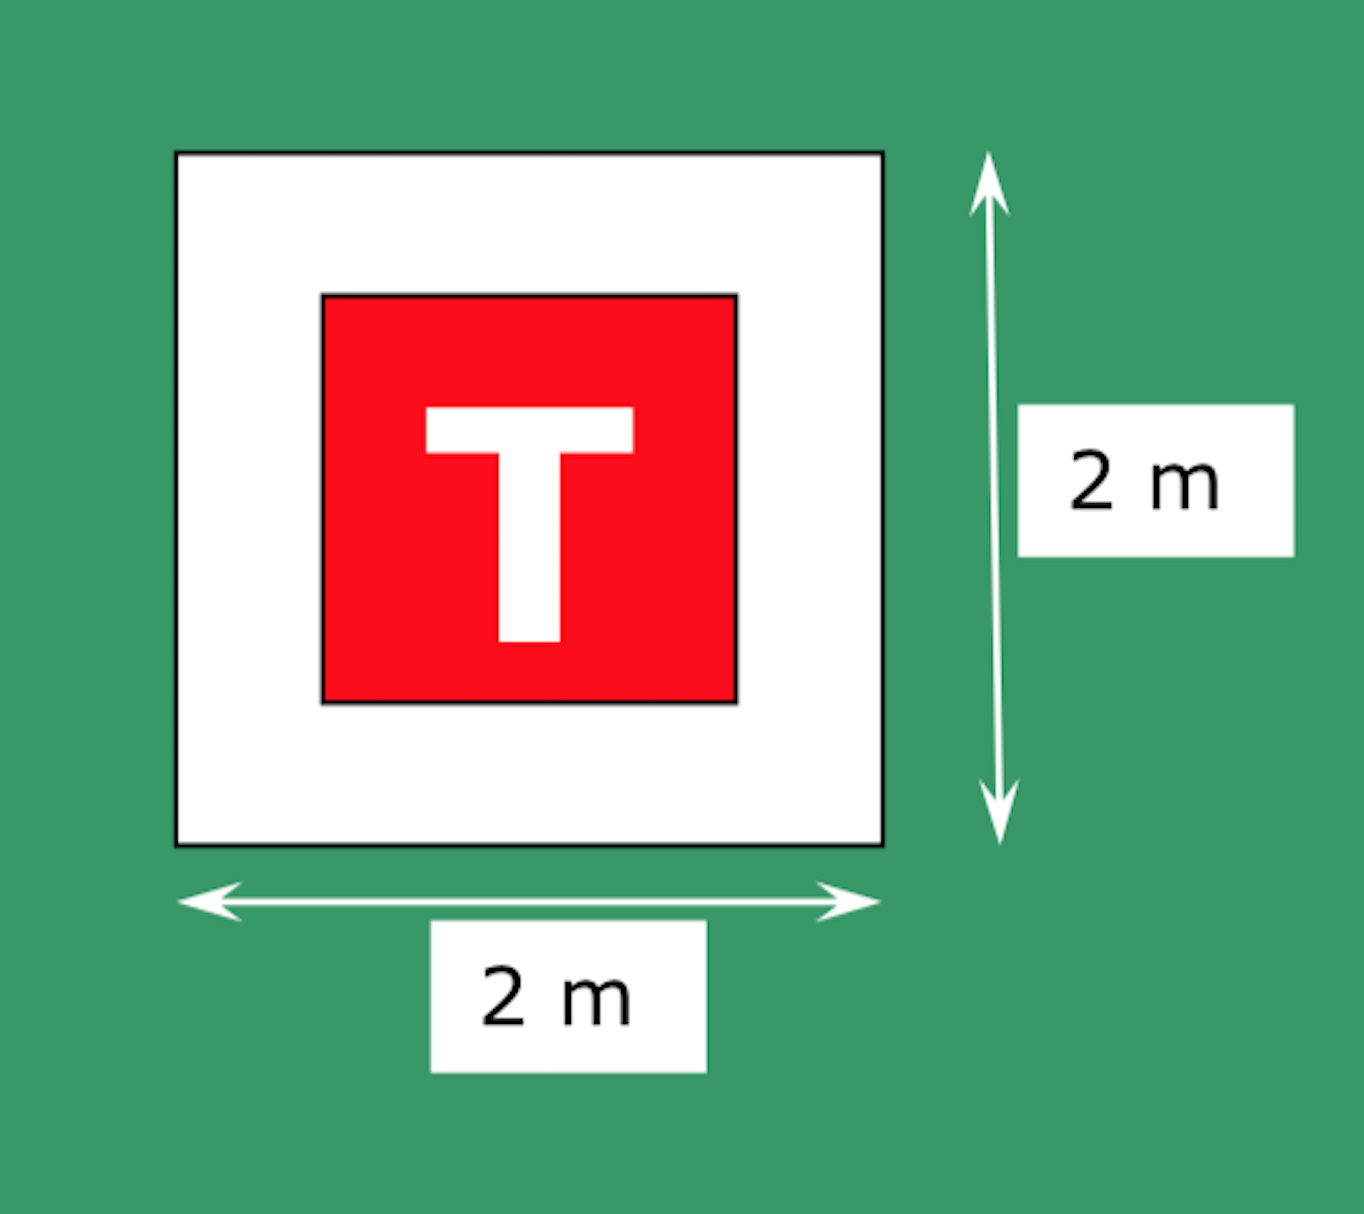
\includegraphics[width=0.48\linewidth]{IMechE_target}
        \caption{Target \cite{IMechE_rules}}
        \label{fig:target}
    \end{center}
\end{wrapfigure}

First, squares are recognised. This is a multi-stage process:
\begin{compactenum}
    \item Convert image to grayscale
    \item Use a Gaussian Blur on the image
    \item Use Canny Edge Detection to find edges
    \item Find complete contours
    \item Find contours that have between 4 and 6 edges
    \begin{compactitem}
        \item \small An ideal square would have 4 edges, but images are rarely perfect.
    \end{compactitem}
    \item Check that the contour is above a minimum size
    \item Check that the solidity of the contour is above a threshold
    \begin{compactitem}
        \item This is done by drawing a rectangle that encloses the entire contour, and comparing the area of the rectangle to the area of the contour
        \item An ideal square would have a solidity of 1
    \end{compactitem}
    \item Check that the aspect ratio of the bounding rectangle is within thresholds
    \item Contours that have passed all of these criteria must be squares
\end{compactenum}
These contours are then drawn onto the image, showing us the squares. This method can be applied to images, or to video by applying it to each frame in the video. It is modified from examples available online.\cite{opencv_tutorials}\cite{pyimagesearch_squares}

\subsubsection{Optical Character Recognition}
Reading the letter inside the target is also a requirement of our system. To this end, Optical Character Recognition (OCR) was added to our system. This is done using the freely available Tesseract OCR library, in conjuction with the pytesseract library that adapts it to Python. A simple function was created that takes an image and puts it through Tesseract, printing all that is written on that page. Once again, it was adapted from examples available online.\cite{pyimagesearch_ocr}

\subsubsection{Target Detection}
The next step was to find the target by finding squares that are conenctric to each other. This was done by finding the coordinates of the center of the square, using OpenCV's \lstinline|moments()| function. This center was then compared to the centers of all other squares that had been found.

At this point, a \lstinline|Square| class was made to improve the code under the concepts of object-oriented programming. A \lstinline|concentric()| method was made in this class that compares squares against each other to see if their center points are within a certain distance of each other (by default, 5\% of the size of the square). Two squares that are concentric are added to a new intance of a \lstinline|Target| class. Repeated comparisons are avoided by using \lstinline|intertools.combinations()| to make a list of all the unique pairs of squares before comparing.

Initially, it appeared that all squares were targets. The problem was discovered to be that there are in fact multiple, very similar squares being generated for each actual square on the image. For example, for a square whose border is a black line might have the outside of the line and the inside of the line counted as seperate squares. These squares are clearly concentric and thus all squares are targets. The problem was solved by creating a \lstinline|similar()| method for \lstinline|Square| and using it to eliminte squares that are too similar (again, 5\% by default), ensuring that all squares are unique before running the \lstinline|concentric()| method to find targets.

From here, it is trivial to calculate the offset of the target from the center of the image or camera frame. This offset will be used as an input into a control system to move the drone above the target.

\subsubsection{Integrating into Control}
Using the code developed in Section \ref{control_implementation}, a program was created to integrate the newly-developed computer vision. This takes off to 10m, and once there the webcam on the computer is turned on. It looks for a target, and uses the offset of the target from the center of the camera as an input for the desired position of the drone. This was verified to work as intended, validating all the work we have done up to this point.

\subsection{Communication}
Communication from Pete to a base station to transmit information will, by necessity, be over a serial connection.

The socat command line utility was used to establish two virtual serial ports which communicate with each other. These are then acessed using the pyserial library to write and read information from these serial ports.

\subsubsection{Serialising Targets}
It was quickly discovered that sending an entire image over a serial connection within a reasonable amount of time is not possible. Even sending the contours of a square does not work well, as this is a large set of points. Thus, it was decided to send only the most important information.

A \lstinline|Square2| and \lstinline|Target2| class were created. These inherit from \lstinline|Square| and \lstinline|Target|. The only difference is that they are missing the contours of the squares. \lstinline|Square| and \lstinline|Target| gained a \lstinline|to_json()| method that converts their attributes to a string using JavaScript Object Notation (JSON), a standard for transmitting information. \lstinline|Square2| and \lstinline|Target2| have a function \lstinline|from_json()| which can recreate the squares from the JSON string.

This was tested by sending the targets over the virtual serial connection, and drawing them on the image. With minor modifications to the way that squares and targets are drawn, this worked sucessfully. Notably, squares are now defined largely based on their bounding rectangle and not on their own contours, which for a square or rectangle makes little difference.

\subsection{Choosing a Computer}
A comparison was made of availible companion computers on the market. The Intel Edison, Raspberry Pi3, Nvidia TX2, Odroid XU4, and Snapdragon Flight were compared on criteria such as processing power, weight, and cost. The full comparison can be seen in Appendix \ref{app:cc_selection}.

Of these, the Raspberry Pi3 was the preffered choice, as it is cheap and light, and has the greatest amount of community support and available documentation. It is, however, borderline as to whether it is powerful to run the required computer vision computation. The Nvidia TX2 is a close second. It is definetely powerful enough to meet our needs, but is significantly more expensive and has less support available. It was therefore decided to buy a Raspberry Pi, and to upgrade to the TX2 if it turns out to not be powerful enough.




%%%%%%%%%%%%%%%%%%%%%%%%%%%%%%%%%%%%%%%%%%%%%%%%%%%%%%%%%%%%%%%%%%%%%%%%%%%%%%%
% APPENDIX
%%%%%%%%%%%%%%%%%%%%%%%%%%%%%%%%%%%%%%%%%%%%%%%%%%%%%%%%%%%%%%%%%%%%%%%%%%%%%%%
\newpage
\appendix
\section{Table of All Symbol Definitions}
\begin{center}
    \emph{Note: values in normal text are constants, values in italics are values derived from constants. Where no value is given, that variable is a dynamic variable which changes continously.}
\begin{longtable}{|ccc|}
    \hline
    \emph{Symbol} & \emph{Definition} & \emph{Value(where appropriate)} \\
    \hline \endhead
    & \emph{Positions and Angles} & \\
    \hline
    $\theta_x$ & Quad Pitch & \\
    $\theta_y$ & Quad Roll & \\
    $\theta_z$ & Quad Yaw & \\
    $\phi_x$ & Jet Pitch & \\
    $\phi_y$ & Jet Roll & \\
    $\phi_z$ & Jet Yaw & \\
    \hline
    & \emph{Dimensions} & \\
    \hline
    $h_f$ & Quad frame height & 5 mm \\
    $r_1$ & Quad frame inner radius & 180 mm \\
    $r_2$ & Quad frame outer radius & 200 mm \\
    $L_R$ & Quad arm length & 100 mm \\
    $r_r$ & Quad arm radius & 2 mm \\
    $r_J$ & Jet radius & 41 mm \\
    $h_J$ & Jet height & 150 mm \\
    $l_c$ & Gimbal servo connecting rod length & 100 mm \\
    \hline
    & \emph{Masses} & \\
    \hline
    $M_{TOT}$ & Total Mass & \\
    $\rho$ & Density of Quad & $2700 kgm^3$ \\
    $M_F$ & Quad frame mass & \\
    $M_R$ & Quad rod mass & \\
    $M_M$ & Motor mass & 50 g \\
    $M_G$ & Gimbal servo mass & 79 g \\
    $M_J$ & Jet mass & \\
    % TODO: add jet mass, explain better
    \hline
    & \emph{Inertias} & \\
    \hline
    $I_{Qx}$ & Quad inertia about x axis & \\
    $I_{Qy}$ & Quad inertia about y axis & \\
    $I_{Qz}$ & Quad inertia about z axis & \\
    $I_{Jx}$ & Jet inertia about x axis & \\
    $I_{Jy}$ & Jet inertia about y axis & \\
    $I_{Jz}$ & Jet inertia about z axis & \\
    \hline
    & \emph{Forces} & \\
    \hline
    $F_x$ & Sum of forces in x direction & \\
    $F_y$ & Sum of forces in y direction & \\
    $F_z$ & Sum of forces in z direction & \\
    $F_{M1}$ & Force from motor 1 & \\
    $F_{M2}$ & Force from motor 2 & \\
    $F_{M3}$ & Force from motor 3 & \\
    $F_{M4}$ & Force from motor 4 & \\
    $F_J$ & Force from jet & \\
    \hline
    & \emph{Torques and Moments} & \\
    \hline
    $\tau_{Qx}$ & Sum of moments on quad about x axis & \\
    $\tau_{Qy}$ & Sum of moments on quad about y axis & \\
    $\tau_{Qz}$ & Sum of moments on quad about z axis & \\
    $\tau_{Gx}$ & Torque of jet gimbal servo about x axis & \\
    $\tau_{Gy}$ & Torque of jet gimbal servo about y axis & \\
    \hline
    & \emph{PID Controllers} & \\
    \hline
    $SP_x$ & Quad X position controller setpoint & \\
    $SP_y$ & Quad Y position controller setpoint & \\
    $SP_z$ & Quad Z position controller setpoint & \\
    $SP_{\theta_x}$ & Quad X angle controller setpoint & \\
    $SP_{\theta_y}$ & Quad Y angle controller setpoint & \\
    $SP_{\theta_z}$ & Quad Z angle controller setpoint & \\
    $O_x$ & Quad X position controller output & \\
    $O_y$ & Quad Y position controller output & \\
    $O_z$ & Quad Z position controller output & \\
    $O_{\theta_x}$ & Quad X angle controller output & \\
    $O_{\theta_y}$ & Quad Y angle controller output & \\
    $O_{\theta_z}$ & Quad Z angle controller output & \\
    $SP_{\phi_x}$ & Jet X angle controller setpoint & \\
    $SP_{\phi_y}$ & Jet Y angle controller setpoint & \\
    $O_{\phi_x}$ & Jet X angle controller output & \\
    $O_{\phi_y}$ & Jet Y angle controller output & \\
    \hline
\end{longtable}
\end{center}

\section{Servo Information} \label{app:servo_info}
Servo information was based on a sample servo that may well end up being used on the vehicle, the Futaba BLS177SV.

\begin{center}
\begin{tabular}{ccc}
    Torque (at 6.6V): & 34 kg-cm \\
    Speed (at 6.6V): & 0.12sec/60\textdegree{} \\
    Weight: & 79g \\
\end{tabular}
\end{center}

We can see from the datasheet that it takes the servo 0.12 seconds to rotate 60\textdegree{}. Assuming it takes 0.01 of those seconds to accelerate to full speed, this gives an acceleration of $873rad/s^2$. Since we know it exerts a torque of 0.34kgm, this means its inertia must be $3.89\times10^{-4}$.
% TODO: perhaps follow this up experimentally?

\section{Thrust to Weight Ratio Calculations} \label{app:thrust_to_weight}
% TODO: add stuff here

\section{Companion Computer Selection} \label{app:cc_selection}
\begin{figure}[h]
    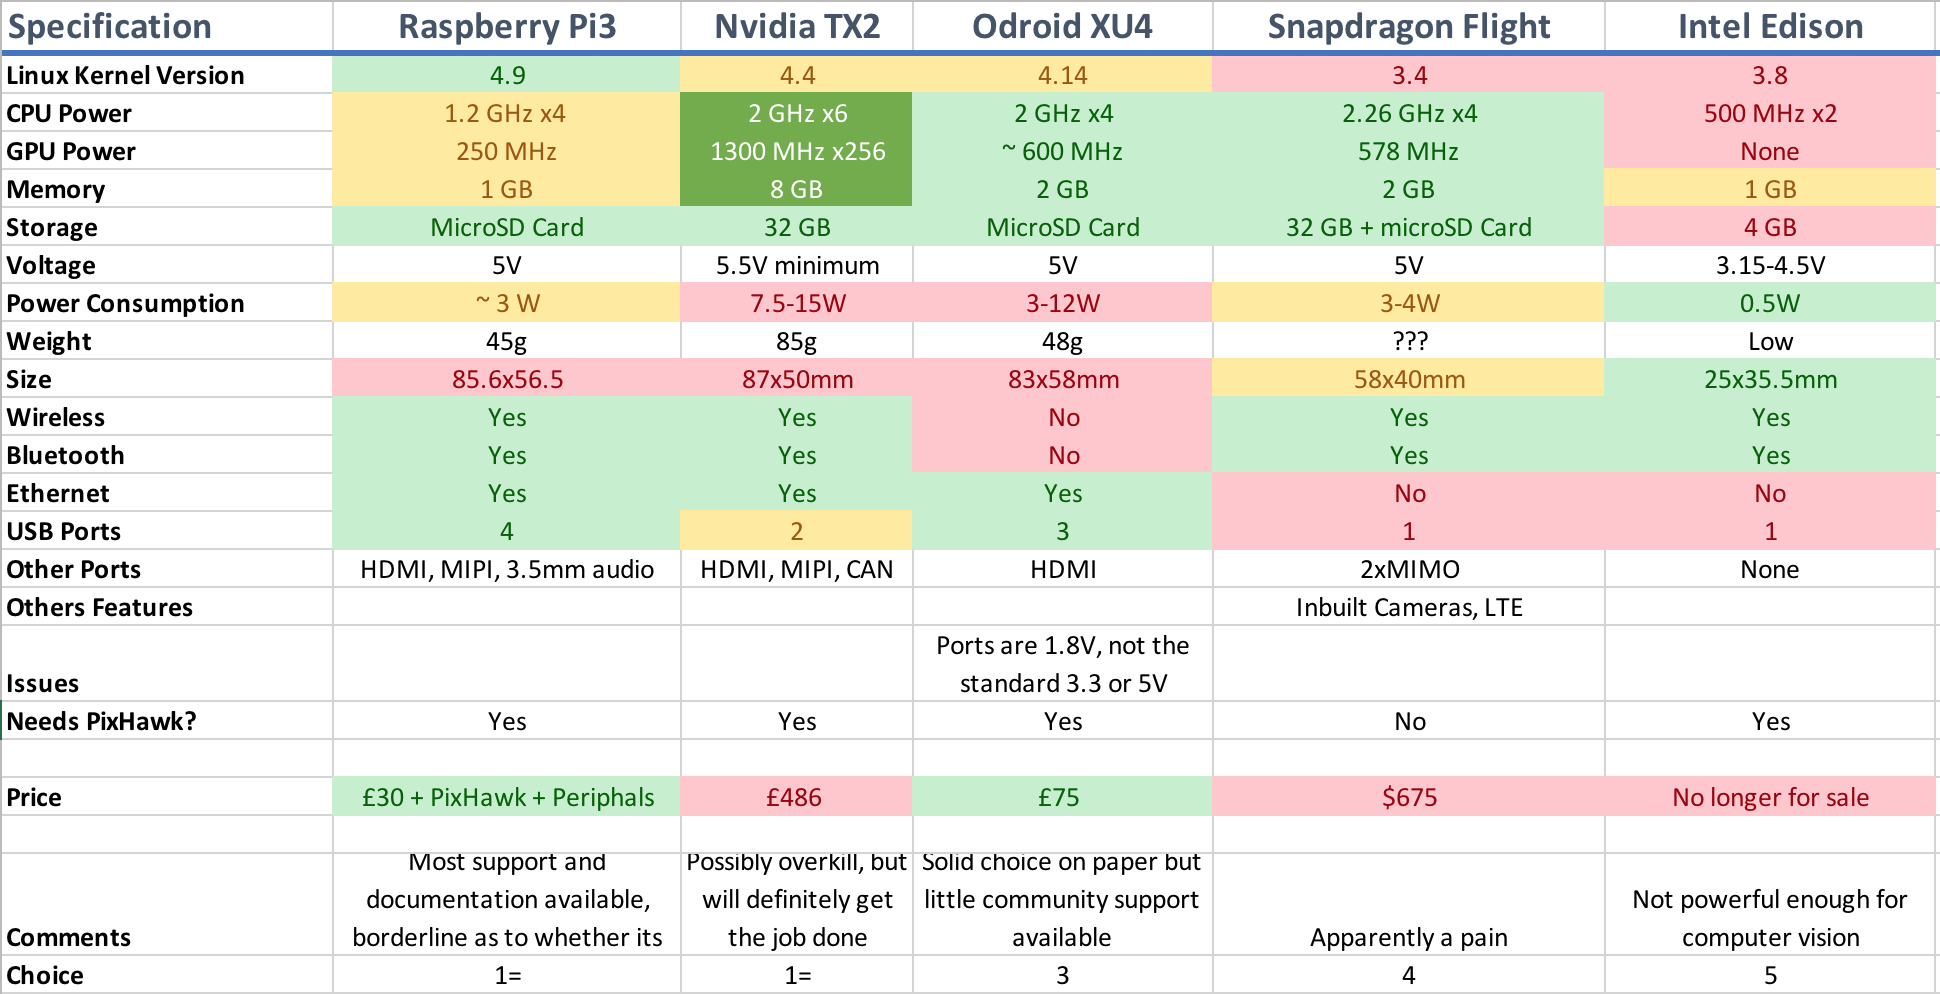
\includegraphics[width=\linewidth]{companion_computer_comparison}
    \caption{}
\end{figure}


%%%%%%%%%%%%%%%%%%%%%%%%%%%%%%%%%%%%%%%%%%%%%%%%%%%%%%%%%%%%%%%%%%%%%%%%%%%%%%%
% BIBLIOGRAPHY
%%%%%%%%%%%%%%%%%%%%%%%%%%%%%%%%%%%%%%%%%%%%%%%%%%%%%%%%%%%%%%%%%%%%%%%%%%%%%%%
\newpage
\begin{thebibliography}{11}

\bibitem{IMechE_about_uas}
    IMechE. About UAS Challenge - IMechE [Internet]. [Accessed 20 December 2017]; Availible from: \url{https://www.imeche.org/events/challenges/uas-challenge/about-uas-challenge}.

\bibitem{IMechE_rules}
    Institution of Mechanical Engineers. University UAS Challenge 2018 Competition Rules [Internet]. Issue 7.1. [Accessed 27 December 2017]; Available from: \url{https://www.imeche.org/docs/default-source/1-oscar/uas-challenge/uas-challenge--competition-rules.pdf?sfvrsn=2}.

\bibitem{PX4_user_guide}
    DroneCode. PX4 Autopilot User Guide [Internet]. Updated 20 December 2017. [Last accessed 20 December 2017]; Availible from: \url{https://docs.px4.io/en/}.

\bibitem{PX4_dev_guide}
    DroneCode. PX4 Development Guide [Internet]. Updated 15 December 2017. [Last accessed 20 December 2017]; Availible from: \url{https://dev.px4.io/en/}.

\bibitem{dronekit}
    3D Robotics. DroneKit-Python Documentation [Internet]. Updated 21 April 2017. [Accessed 20 December 2017]; Available from: \url{http://python.dronekit.io}.

\bibitem{opencv_tutorials}
    OpenCV. OpenCV-Python Tutorials — OpenCV 3.0.0-dev documentation [Internet]. Last updated 10 Novemeber 2014. [Accessed 22 December 2017]; Available from: \url{https://docs.opencv.org/3.0-beta/doc/py_tutorials/py_tutorials.html}.

\bibitem{pyimagesearch_squares}
    Adrian Rosebrock. Target acquired: Finding targets in drone and quadcopter video streams using Python and OpenCV [Internet]. 4 May 2015. [Accessed 22 Decemeber 2017]; Available from: \url{https://www.pyimagesearch.com/2015/05/04/target-acquired-finding-targets-in-drone-and-quadcopter-video-streams-using-python-and-opencv/}.

\bibitem{pyimagesearch_ocr}
    Adrian Rosebrock. Using Tesseract OCR with Python [Internet]. 10 July 2017. [Accessed 22 December 2017]; Available from: \url{https://www.pyimagesearch.com/2017/07/10/using-tesseract-ocr-python/}.


\end{thebibliography}

\end{document}
